\chapter{Arquitectura e implementación da aplicación}
\label{chap:implementacion_aplicacion}
Detalles da implementación do software, problemas xurdidos e solucions aplicadas
posibles subseccion:
servidor python- control das luces, control da camara, comunicacion, sockets e broadcasting
aplicacion android- layouts e botons, comunicacions ordes e recepcion de video, xestion de varios dispositivos


\textcolor{red}{Estou algo preocupado, porque agora mesmo o SW é moi sinxelo (literalmente 4 páxinas ...)}


Son moitas as posibilidades de implementación deste dispositivo, os requisitos principais son:
\begin{itemize}
    \item Dispoñer dunha pantalla para visualizar o vídeo e o estado das luces.
    \item Contar con algunha interface de entrada de datos como botóns ou pantalla táctil.
    \item Dispoñer dun hardware para comunicarse co dispositivo principal. Como por exemplo: Wi-Fi, Bluetooth ou USB.
    \item Contar cunha batería ou fonte de alimentación
\end{itemize}

Realizar unha implementación física do dispositivo contaria coas vantaxes de poder contar cunha alta personalización dos seus compoñentes e robustez ao contar cun unico dispositivo obxetivo. Sen embargo se nos presenta outra opción moito máis atractiva: utilizar un telefono móbil e crear unha aplicacíon dende onde poder visualizar o vídeo e controlar as luces, aparte de aforrar a construción do dispositivo. Reduciremos así o número de compoñentes que o usuario ten que levar, xa que é habitual dispoñer dun móbil en todo momento.

Desarrollaremos a aplicación para o sistema operativo Android xa que este é o sistema operativo máis empregado globalmente e nos permitirá chegar a un maior numero de usuarios.

Para suxeitar un teléfono móbil ao manillar da bicicleta existen múltiples anclaxes que se adaptan a varios tamaños de teléfono. Tamén existen plantillas configurables segundo o tamaño do teléfono que despois se poden imprimir en 3D.

\section{Esquema xeral da aplicación}
Para crear esta aplicación android optarase por utilizar a linguaxe de programación Kotlin e a o entorno de programación Android Studio. Kotlin é unha linguaxe de programación creada por JetBrains cun obxetivo inicial de executarse na maquina virtual de Java, dende 2017 Kotlin é unha linguaxe oficial para desenvolver apicacións android.

Algunhas das suas vantaxes fronte a Java son:
\begin{itemize}
    \item Unha maior expresividade: Podes escribir mais con menos código.
    \item Maior seguiridade: En Kotlin e obligatorio especificar a nulabilidade dos obxetos e esta se comproba en tempo de compilación.
    \item É funcional: Kotlin é unha linguaxe orientada a obxetos pero inclue conceptos da programación funcional como as expresións lambda.
    \item Fai uso de extensión de funcións: Permite extender clases con novas funcionalidades se necesidade de ter aceso o codigo da clase.
    \item É altamente interoperable: Podese utilizar librerias e  clases de java no mesmo proxento.
\end{itemize}
incluir referencia a libro kotlin

A aplicación contará con catro compoñentes. O principal será a MainActivity, a encargada de iniciar as compoñentes a visualizar na pantalla, executar as ordes e monstrar a información. O segundo será o layout onde se definiran as compoñentes a visualizar e a sua posición en pantalla. O terceiro a clase request a encargada da conexión co servidor e de trasmitirlle as ordes. O cuarto elemento é a clase encargada de recibir o video e decodificalo.

\section{Actividade principal}
A actividade principal ou MainActivity dunha aplicación android é a primeira pantalla que aparece cando executamos a aplicación e a encadgada de controlar o seu funcionamento e a sua interface de usuario. Neste caso a actividade será a encargada de mostrar os botóns e encargarse do seu funcionamento, amosar o estado da conexión, encargarse da xestión do sensores e reproducir o video. O mesmo tempo encagarase de instanciar e comunicarse coas clases encargadas da conexión co dispositivo e da recepción de video.

\subsection{Layout}
Un layout é a definición da estrutura da interface de usuario. Esta actividade contará con dous layouts un para a posición vertical e outro para a posición orizontal da pantalla
\subsubsection{Layout vertical}
Este layout contará cunha superficie reservada para o video na metade superior da pantalla. Na metade inferior situaranse os botóns encargados de executar as ordes. Na parte superior situase a barra de estado que na sua parte dereita contará cun botón para conectar que servirá o tempo de indicador de conexión, a sua esquerda mostrarase unha barra para controlar a intensidade dos leds.

imaxes layout vertical
\subsubsection{Layout horizontal}
Neste layout o video mostrarase como o fondo e os botóns sobre él. Os de xiro a esquerda e xiro dereita situadso a ambolosdous lados e o resto incluindo o de control de intensidade lumínica e o de conexión situaranse na parte de inferior da pantalla.

imaxes layout horizontal
\subsection{Ciclo de vida da actividade}
En android cada actividade conta conta cun ciclo de vida, pasa por vairos estados dende antes de iniciarse ata despois de finalizar. O estado principal dunha actividade é activa, no momento que a actividade está en primeiro plano e interactuando co usuario.

imaxe ciclo actividade

Para xestionar o que sucede no resto de estados utilizanse unhas funcións de callbacks, no noso caso realizaremos as seguintes accións en cada fase:
\subsubsection{onCreate}
Este método e o que se chama ao executar a actividade. Nel iniciaremos os compoñentes a mostrar en pantalla e definiremos o seu comportamento.

Aquí xestionaremos o estado da conexión, iniciando a clase request se non esta en funcionameto e enviando mensaxes o dispositivo para comprobar que segue conectado. Tamén xestionaremos o estado da transmisón de video xa que será necesario iniciar a recepción antes de iniciar a transmisión.
\subsubsection{onResume}
Este método executase despois de onCreate cando a pantalla xa é visible para o usuario.

Resxistrarase aquí un sensor listener para obter a información do sensor de luz.
\subsubsection{onPause}
Este método executase cando a aplicación deixa de estar en primer plano, se o usuario a minimiza u otra aplicación executase a actividade pasará a onStop se despois de aceder a aplicaciós recentes a aplicación volve a primer plano pásese o metodo onResume.

No noso caso neste método cancelaremos o rexistro do sensor xa que non se seguira a utilizar e deteremos a transmisión de video se se esta a executar.
\subsubsection{onDestroy}
Neste método a actividade e detida completamente e devense livera os recuros.

Aqui enviaremos a orde para deter a conexión co dispositivo.

\subsection{Botones}
A actividade é a encargada de iniciar os botóns e manexar o seu funcionamento. Estes botón son os seguintes:
\begin{itemize}
    \item \textbf{Esquerda:} O pulsar este botón enviaráse unha orde de acender a luz de xiro a esquerda. Se hai algunha luz acesa se enviará primeiro unha orde para apagalas. O pulsalo por segunda vez se enviara a orde de apagar luz de xiro e no caso de que a luz vermella estivese acesa antes de indicar o xiro esta luz se acenderá de novo. O botón palpebrará en amarelo mentres estea aceso.
    \item \textbf{Dereita:} O seu funcionamento é o mesmo que no botón esquerda.
    \item \textbf{Vermello:} O pulsalo enviarase unha orde para acender a luz de vermella, o bonton non funcionara se algunha das luces de xiro está acesa.
    \item \textbf{Noite:} O pulsalo activarase o modo noite, no que o sensor lumínico do móbil encargaráse de acender a luz vermella cando a luz ambien baixe de certo umbral.
    \item \textbf{Freo:} Activa o modo de freada no que acenderase a luz vermella progresivamente cando o acelerometro do dispositivo movil detecte unha freada.
    \item \textbf{Brillo:} Este botón despregará unha barra cun indicador que poderemos deslizar para elexir a inntesidade das luces
    \item \textbf{Conexión:} Este botón enviará unha orde de conexión, unha vez conectado cambiará a súa apariencia para indicar que exite conexión co dispositivo.
\end{itemize}
\subsection{Sensores}
Unhas das ventaxa de utilixar un dispositivo mobil é que estes contan con diversos sensores para moitos fins. No noso caso utilizarase o acelereometro e o xiroscopio para resixistrar cambios na posición e acelercaións no dispositivo e o sensor de luz para medir a intensidade de luz no ambiente.
En android acederemos o sensor instanciando a clase SensorManager e definindo unha instancia do sensor da que obteremos os datos mediante a función on sensor change
\subsubsection{Acelerometro}
\subsubsection{Sensor de Luz}
O sensor de luz é un fotorreceptor que xenera unha sinal electrica dependendo da incidencia de fotóns. Para utilizar o sensor rexistraermos un sensor listener no metodo onResume e o metodo de callback onSensorChanged executarase cada vez que se detecte un cambio, neste metodo definirase o comportamente do sensor: Cando o botón de Noite esta activado encenderase o botón Vermello se o sensor rexistra un valor inferior a 400 lumines. Este valor correspondese coa intensidade lumínica o comenzo do solpor.
incluir referenciaaa

\subsection{Superficie de video}
Iniciarase a superficie de video na fase de creación da aplicación, procederase a reflexar a superfice para facer un efecto de espello para facer mais natural a a visualización do video. O video asignarase a superficie iniciando a clase VideoReceiver mediante as funcións de callback que se executarán cando se produza un cambio na superfice de video.

\section{Comuniciacíon co dispositivo}
Crearase unha clase Request encargada de todalas comunicacións co dispositivo.  Esta clase, unha vez instanciada, encargarase de establecer a conexión co dispositivo, reconectar se se perde a conexión e transmitirlle as ordes.

\subsection{Broadcast}
Para coñecer a direción ip do servidor, a clase request conta cunha función que abrirá un socket no porto 5555 para esperar a recepción dun datagrama broadcasteado a todaslas direcións. O recibir o datagrama comprobase que conten a mensaxe "BikeView" se é asi a función devolverá a direción ip emisora do paquete.

\subsection{Conexión}
Unha vez obtida a direción ip a clase request utilizará unha función para establecer a conexión que devolverá un socket conectado ao socket remoto do servidor.

\subsection{Transmisión de ordes}
Para transmitir as ordes a clase request contara cunha función que recive a mensaxe a transmitir e a envía atraves do socket. Espera a recibir respota do servidor e se é positiva devolve o valor booleano verdadeiro, en caso de non recibila devolve o valor falso.

\section{Recepción de video}
Para este apartado crearase a clase VideoReceiver encargarase
O video é transmitido codificado no formato H.264

\section{Anclaxe a bicicleta}
Existén diversas opcións paras suxeitar o móbil o guiador dunha bicicleta, no mercado hai soportes para dispositivos concretos e outros que se adaptan ao tamaño e forma de diferentes modelos. No noso caso utilizaremos unha codigo SCAD que executaremos co software de deseño 3D paramétrico OpenSCAD no que introduciremos as dimensións do dispositivo e como resultado obetremos un arquivo STL co deseño 3D do soporte.
\begin{figure}[tb]
  \centering
  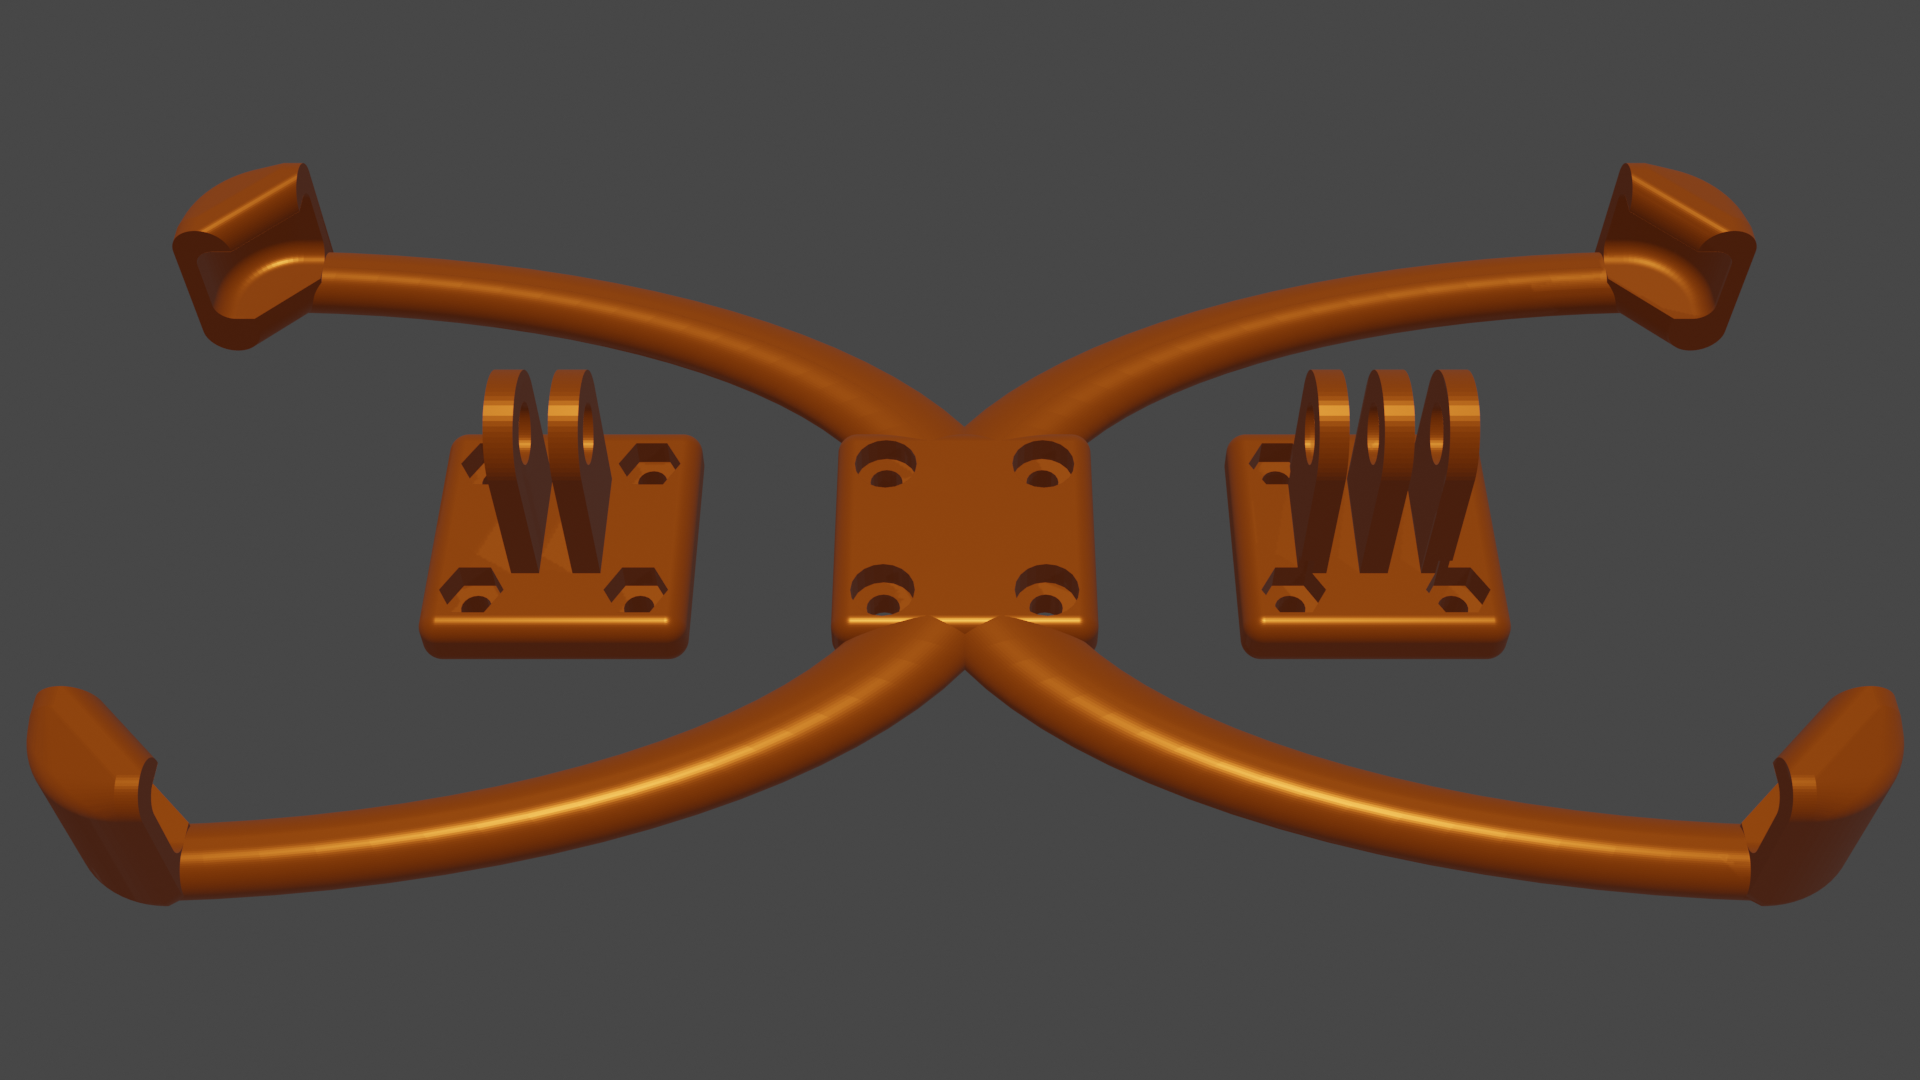
\includegraphics[scale=.2]{imaxes/soporte-mobil.png}
  \caption{Desño 3D do soporte para o dispositivo móbil.}
  \label{f:soporte móbil}
\end{figure}
Vendo que os soportes impresos non constaban coa resistencia esperada optouse por utilizar un soporte de aluminio nas probas para preservar a integridade do dispositivo móbil.
